\documentclass{homework}
\usepackage[spanish]{babel}
% Paquetes para incluir figuras generadas por las simulaciones
\usepackage{graphicx}
\usepackage{float}
\decimalpoint

\author{José Ángel Aké}
\class{Teoría cuántica de campos y materia condensada}
\date{\today}
\title{Ejercicio extra: Modelo SSH}
\address{Posgrado en Ciencias Físicas, UNAM}
\setunitname{Pregunta}

\begin{document}  
\maketitle

% Referencias
\section*{Resultados del modelo SSH (Su-Schrieffer-Heeger)}
Los resultados mostrados a continuación fueron obtenidos con la simulación del modelo SSH implementada en el cuaderno de Julia. Se incluyen (i) el espectro completo de energías en función del parámetro intercelular $t_2 /t_1$, y (ii) el conteo de estados de borde localizados en los extremos de la cadena.

\begin{figure}[H]
    \centering
    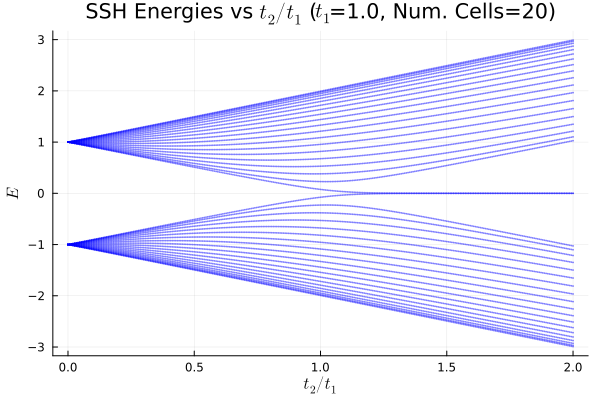
\includegraphics[width=0.49\textwidth]{../ssh_full_spectrum_vs_t2.png}
    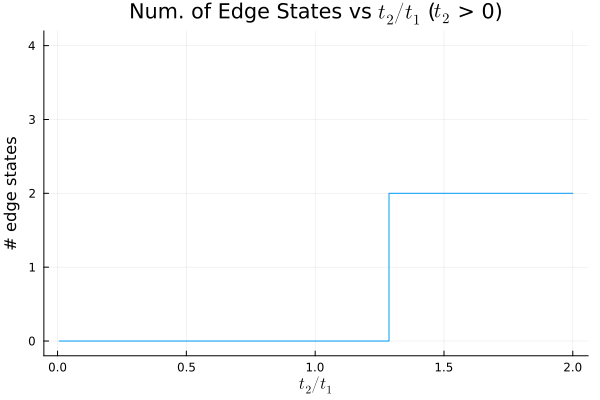
\includegraphics[width=0.49\textwidth]{../ssh_edgecount_vs_t2.png}
    \caption{Izquierda: Espectro completo de energías vs $t_2/t_1$ para una cadena SSH con condiciones de borde abiertas (parámetros: Ncells=20, $t_1=1.0$). Se observan las bandas del bulk (estados extendidos) que se abren con un gap en $t_2/t_1=1$, y puntos en $E\approx0$ correspondientes a estados de borde en la fase topológica ($t_2/t_1 > 1$). 
    Derecha: Número de estados de borde vs $t_2/t_1$ (mismos parámetros). El conteo es 0 en la fase trivial ($t_2/t_1 < 1$) y salta a 2 en la fase topológica ($t_2/t_1 > 1$), reflejando la transición topológica del modelo SSH.}
    \label{fig:ssh_results}
\end{figure}

Notar que: El modelo SSH describe una cadena unidimensional dimerizada con \textit{hopping} intracelular $t_1$ y intercelular $t_2$. La transición topológica ocurre en $t_2/t_1 = 1$, donde aparecen estados de borde de energía cero, localizados en los extremos para $t_2 > t_1$. Los resultados numéricos confirman la estructura de bandas y la presencia de estados de borde, alineándose con la teoría analítica.

% Referencias
%\bibliographystyle{plain}
%\bibliography{citations}

\end{document}

